\subsection{Residual-score $M=8$: combined datasets}

Across 120 paired conditions, residual-score PRISM-XAI transmits 242.52 kbit on average versus 243.71 kbit for MAP-XAI-only. The $1.19\pm0.41$ kbit reduction is statistically detectable but operationally small (0.50\%). Coverage changes by only $+0.021$ percentage points and critical recall by $-0.039$ points. This configuration therefore establishes reproducibility and near-equivalence of the two proposed layers, not a large scheduling gain.

The five figures explain that small aggregate difference. The traces show similar sparse-release behavior for PRISM-XAI and MAP-XAI-only; the fairness panels place both in the same high-fairness region. The privacy--fidelity and Pareto plots show that fixed-DP and full-packet policies use much more traffic but also occupy different service regions, so they cannot support a matched comparison. Top-$K$ overlap is above random in the combined analysis, driven by OPSD rather than UCI. The ablation panels show only a 1.46\% traffic gain from adaptive resolution in this configuration.

\begin{figure*}[p]
\centering
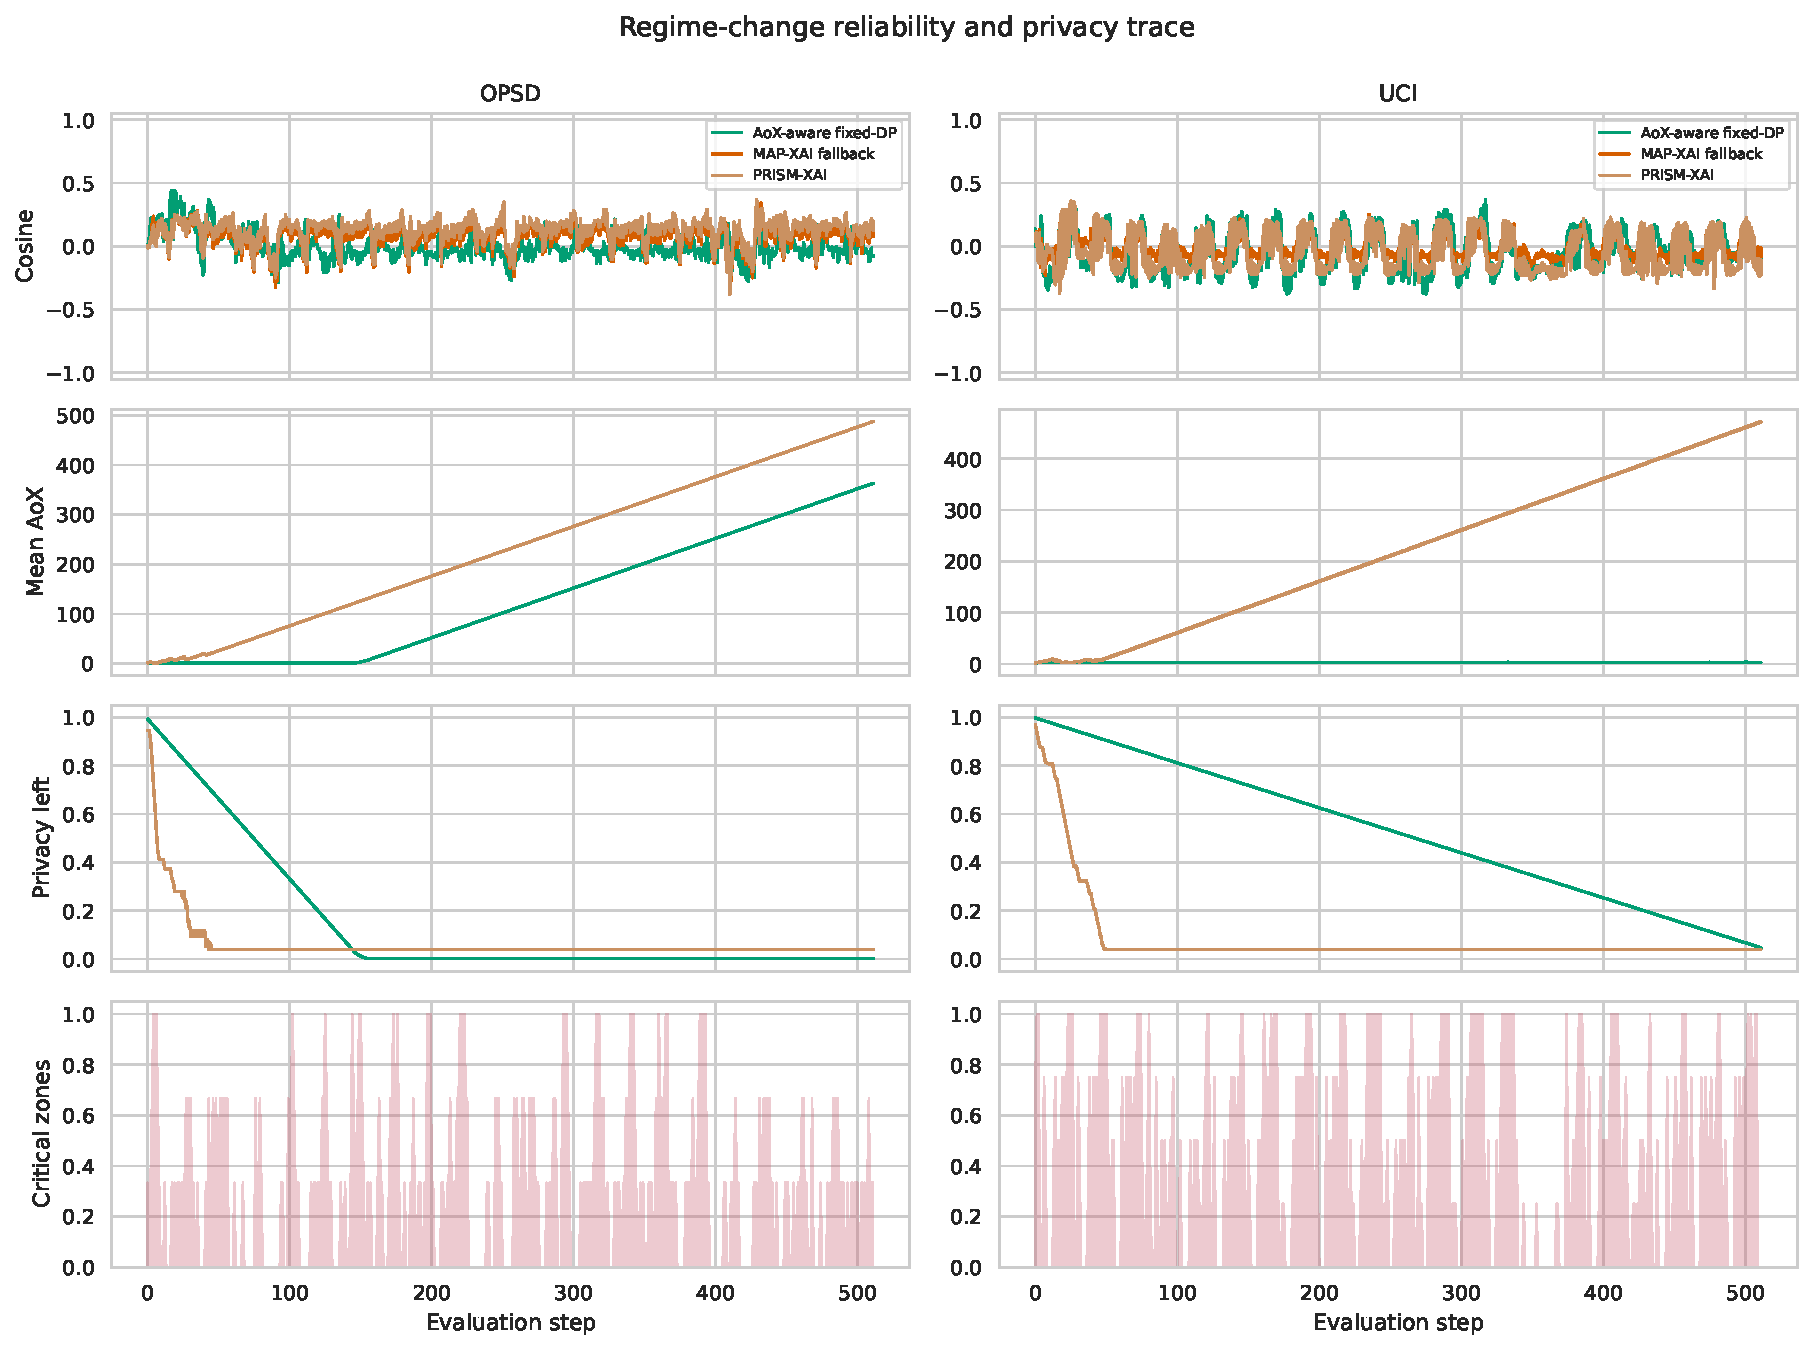
\includegraphics[width=0.96\textwidth,height=0.82\textheight,keepaspectratio]{supplementary_figures/residual_m8_combined_regime_trace.pdf}
\caption{Residual-score $M=8$, combined datasets: representative regime trace. The interpretation and claim boundary are given in the preceding subsection discussion.}
\end{figure*}
\clearpage

\begin{figure*}[p]
\centering
\includegraphics[width=0.96\textwidth,height=0.82\textheight,keepaspectratio]{supplementary_figures/residual_m8_combined_fairness_reliability.pdf}
\caption{Residual-score $M=8$, combined datasets: fairness and reliability. The interpretation and claim boundary are given in the preceding subsection discussion.}
\end{figure*}
\clearpage

\begin{figure*}[p]
\centering
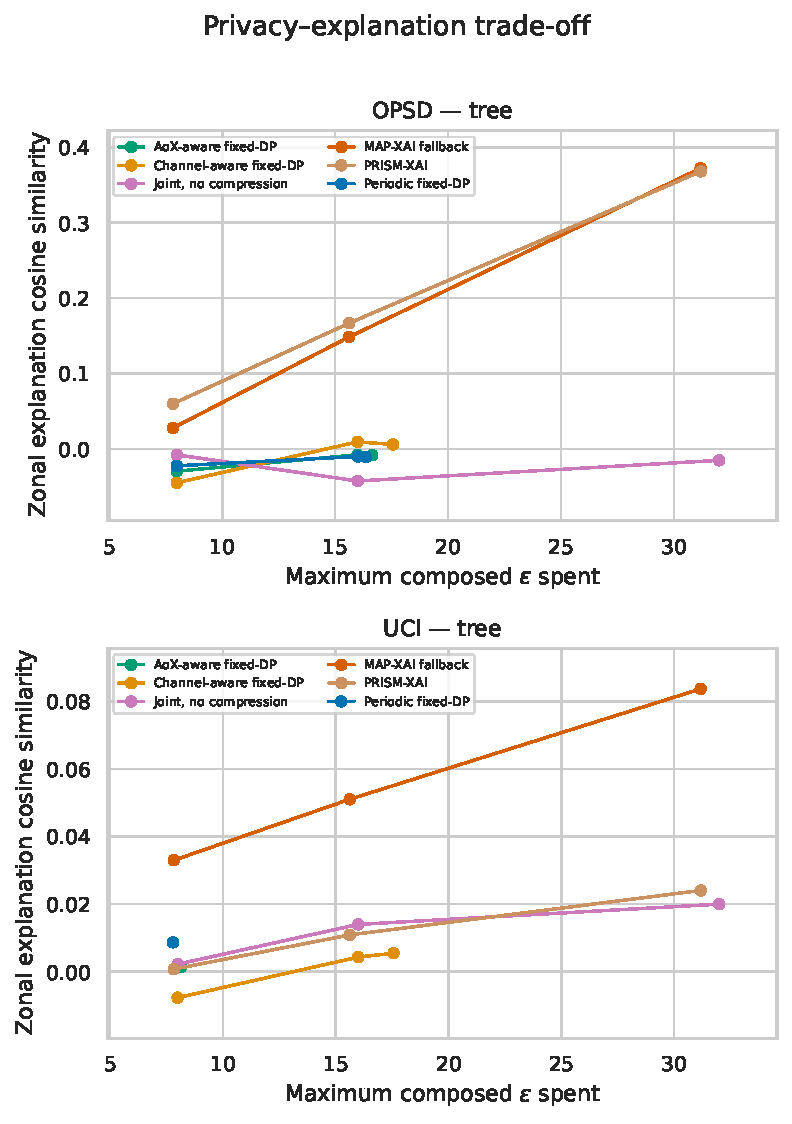
\includegraphics[width=0.96\textwidth,height=0.82\textheight,keepaspectratio]{supplementary_figures/residual_m8_combined_privacy_fidelity.pdf}
\caption{Residual-score $M=8$, combined datasets: privacy and fidelity. The interpretation and claim boundary are given in the preceding subsection discussion.}
\end{figure*}
\clearpage

\begin{figure*}[p]
\centering
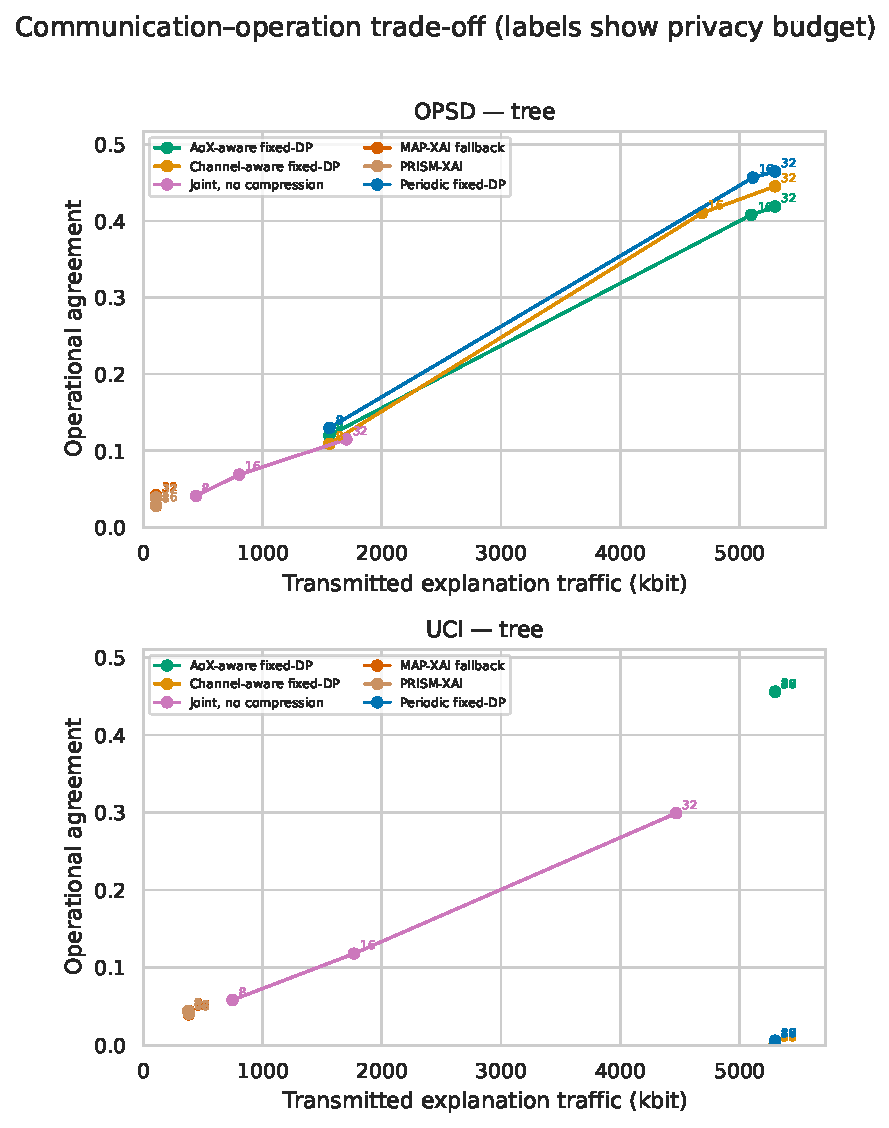
\includegraphics[width=0.96\textwidth,height=0.82\textheight,keepaspectratio]{supplementary_figures/residual_m8_combined_pareto_bits_fidelity.pdf}
\caption{Residual-score $M=8$, combined datasets: traffic--fidelity Pareto analysis. The interpretation and claim boundary are given in the preceding subsection discussion.}
\end{figure*}
\clearpage

\begin{figure*}[p]
\centering
\includegraphics[width=0.96\textwidth,height=0.82\textheight,keepaspectratio]{supplementary_figures/residual_m8_combined_ablation_results.pdf}
\caption{Residual-score $M=8$, combined datasets: ablation results. The interpretation and claim boundary are given in the preceding subsection discussion.}
\end{figure*}
\clearpage

\subsection{Residual-score $M=8$: OPSD}

On OPSD, PRISM-XAI uses about 104--106 kbit across the displayed budgets, while periodic fixed-DP rises from roughly 1.56 Mbit at $\epsilon_{\max}=8$ to 5.11 Mbit at $\epsilon_{\max}=16$. This is not an equal-service comparison: PRISM coverage is about 0.071, whereas the periodic operating point increases from about 0.278 to 0.985. The figures should therefore be read as a traffic--service frontier, not as evidence that the lowest-traffic point universally dominates.

OPSD provides the clearest positive fidelity signal. Across the paired study, Top-$K$ overlap exceeds the random reference by $0.0668\pm0.0265$, with multiplicity-adjusted support. The privacy--fidelity panels nevertheless show substantial uncertainty and no monotone guarantee for every explainer and budget. The high Jain values indicate that selective release is distributed relatively evenly across endpoints, while the trace and ablation panels show that compression and abstention, rather than channel opportunism alone, create the low-traffic operating point.

\begin{figure*}[p]
\centering
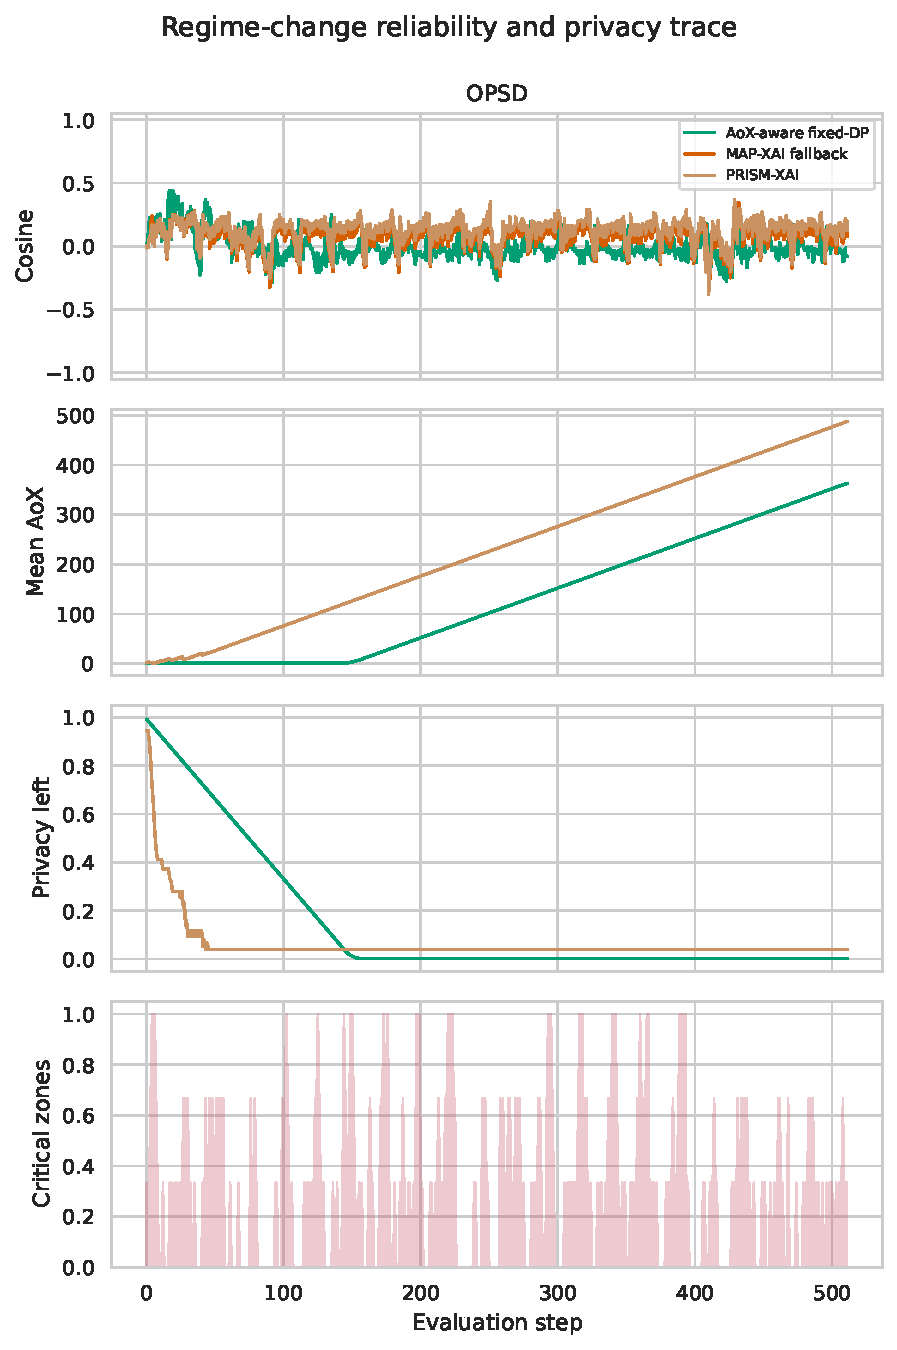
\includegraphics[width=0.96\textwidth,height=0.82\textheight,keepaspectratio]{supplementary_figures/residual_m8_opsd_regime_trace.pdf}
\caption{Residual-score $M=8$, OPSD: representative regime trace. The interpretation and claim boundary are given in the preceding subsection discussion.}
\end{figure*}
\clearpage

\begin{figure*}[p]
\centering
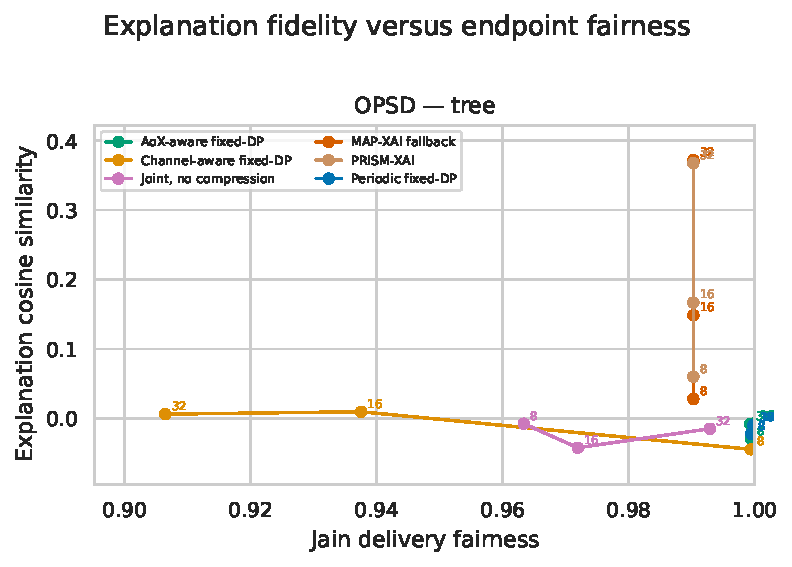
\includegraphics[width=0.96\textwidth,height=0.82\textheight,keepaspectratio]{supplementary_figures/residual_m8_opsd_fairness_reliability.pdf}
\caption{Residual-score $M=8$, OPSD: fairness and reliability. The interpretation and claim boundary are given in the preceding subsection discussion.}
\end{figure*}
\clearpage

\begin{figure*}[p]
\centering
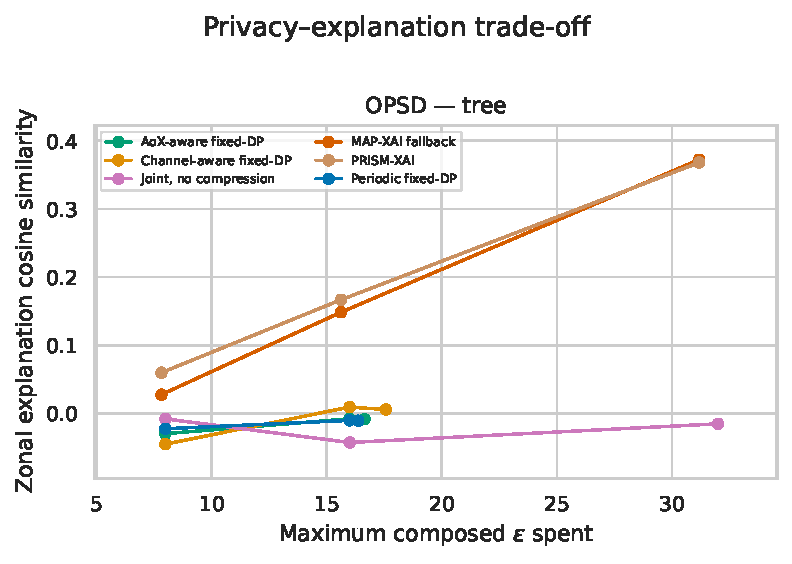
\includegraphics[width=0.96\textwidth,height=0.82\textheight,keepaspectratio]{supplementary_figures/residual_m8_opsd_privacy_fidelity.pdf}
\caption{Residual-score $M=8$, OPSD: privacy and fidelity. The interpretation and claim boundary are given in the preceding subsection discussion.}
\end{figure*}
\clearpage

\begin{figure*}[p]
\centering
\includegraphics[width=0.96\textwidth,height=0.82\textheight,keepaspectratio]{supplementary_figures/residual_m8_opsd_pareto_bits_fidelity.pdf}
\caption{Residual-score $M=8$, OPSD: traffic--fidelity Pareto analysis. The interpretation and claim boundary are given in the preceding subsection discussion.}
\end{figure*}
\clearpage

\begin{figure*}[p]
\centering
\includegraphics[width=0.96\textwidth,height=0.82\textheight,keepaspectratio]{supplementary_figures/residual_m8_opsd_ablation_results.pdf}
\caption{Residual-score $M=8$, OPSD: ablation results. The interpretation and claim boundary are given in the preceding subsection discussion.}
\end{figure*}
\clearpage

\subsection{Residual-score $M=8$: UCI}

UCI has more endpoints and therefore higher absolute PRISM traffic: approximately 373--381 kbit in the displayed conditions. Periodic fixed-DP is near 5.30 Mbit, but it operates at very different coverage and recall. PRISM maintains a sparse selective-release regime with coverage near 0.09 in the shown conditions; this low service level must remain visible when interpreting its communication efficiency.

The UCI fidelity conclusion is weaker than OPSD. The paired Top-$K$ difference from random is $-0.0097\pm0.0234$ and is not detected by either adjusted test. Consequently, the fairness and Pareto figures support a communication-allocation interpretation, but not a claim that the transmitted feature sets are reliably more informative than random selection on UCI. The regime traces also show that additional privacy allowance does not automatically repair this limitation.

\begin{figure*}[p]
\centering
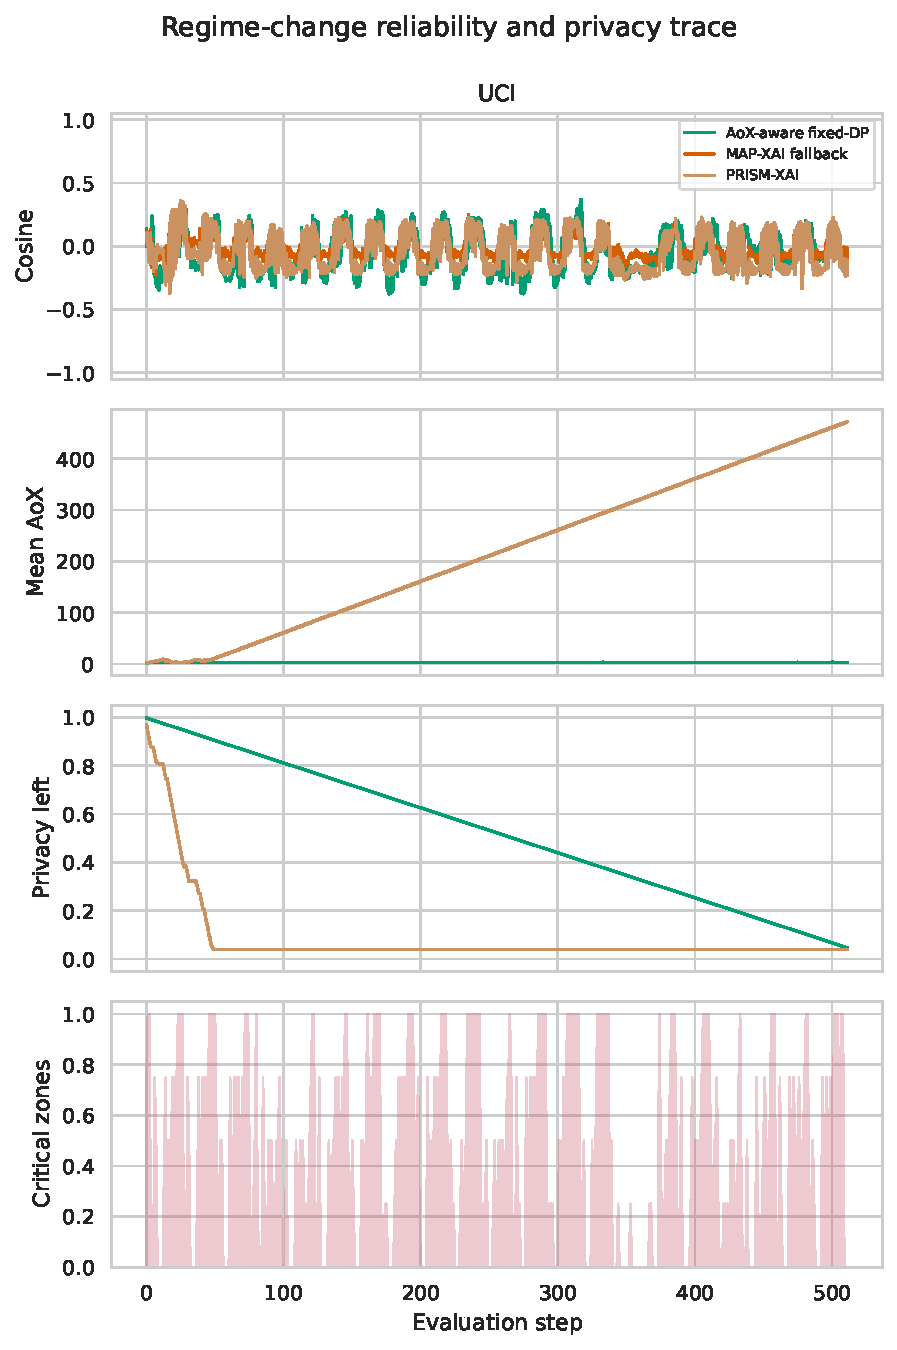
\includegraphics[width=0.96\textwidth,height=0.82\textheight,keepaspectratio]{supplementary_figures/residual_m8_uci_regime_trace.pdf}
\caption{Residual-score $M=8$, UCI: representative regime trace. The interpretation and claim boundary are given in the preceding subsection discussion.}
\end{figure*}
\clearpage

\begin{figure*}[p]
\centering
\includegraphics[width=0.96\textwidth,height=0.82\textheight,keepaspectratio]{supplementary_figures/residual_m8_uci_fairness_reliability.pdf}
\caption{Residual-score $M=8$, UCI: fairness and reliability. The interpretation and claim boundary are given in the preceding subsection discussion.}
\end{figure*}
\clearpage

\begin{figure*}[p]
\centering
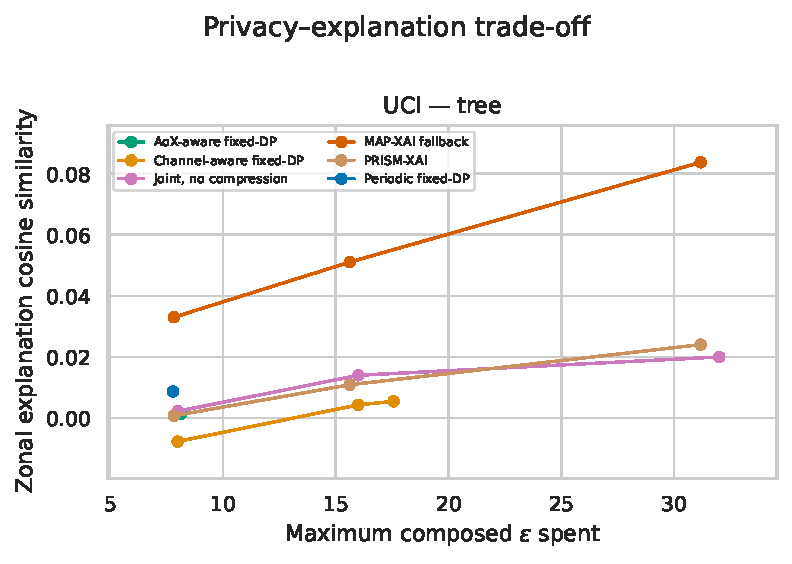
\includegraphics[width=0.96\textwidth,height=0.82\textheight,keepaspectratio]{supplementary_figures/residual_m8_uci_privacy_fidelity.pdf}
\caption{Residual-score $M=8$, UCI: privacy and fidelity. The interpretation and claim boundary are given in the preceding subsection discussion.}
\end{figure*}
\clearpage

\begin{figure*}[p]
\centering
\includegraphics[width=0.96\textwidth,height=0.82\textheight,keepaspectratio]{supplementary_figures/residual_m8_uci_pareto_bits_fidelity.pdf}
\caption{Residual-score $M=8$, UCI: traffic--fidelity Pareto analysis. The interpretation and claim boundary are given in the preceding subsection discussion.}
\end{figure*}
\clearpage

\begin{figure*}[p]
\centering
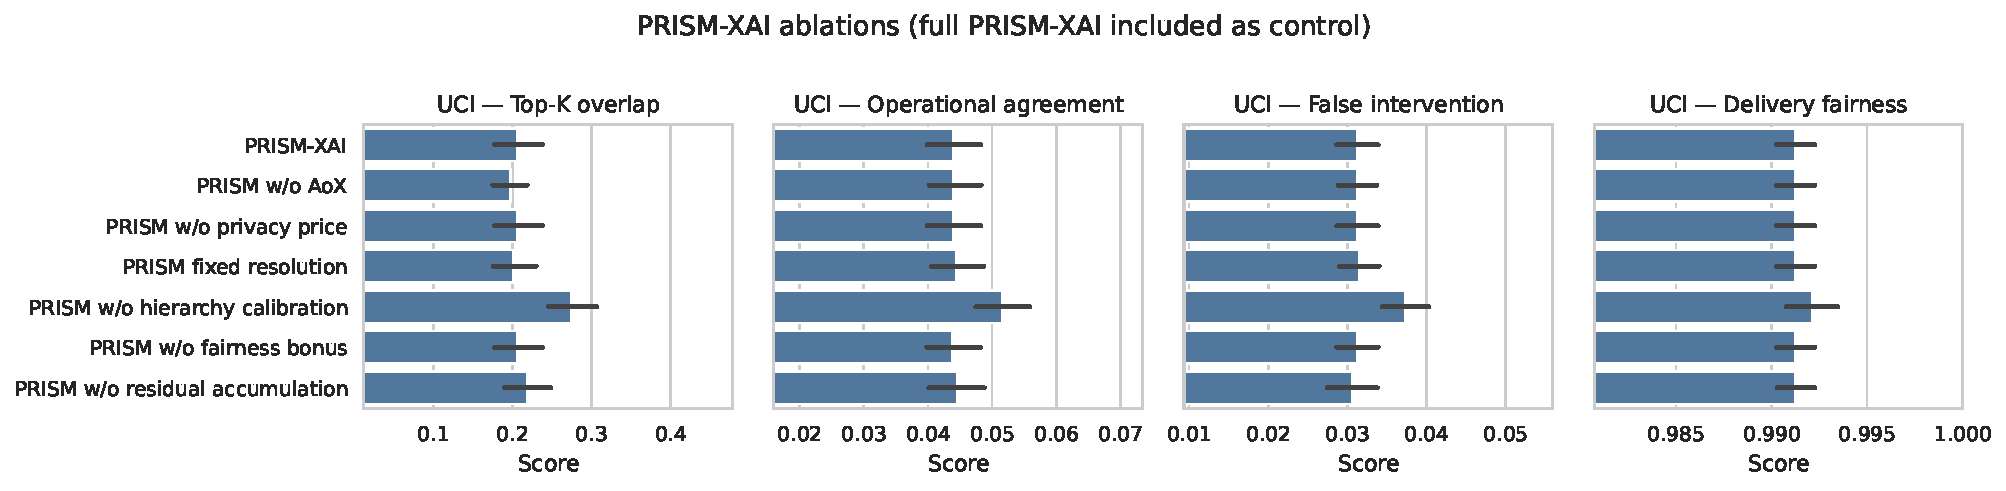
\includegraphics[width=0.96\textwidth,height=0.82\textheight,keepaspectratio]{supplementary_figures/residual_m8_uci_ablation_results.pdf}
\caption{Residual-score $M=8$, UCI: ablation results. The interpretation and claim boundary are given in the preceding subsection discussion.}
\end{figure*}
\clearpage

\subsection{Residual-score $M=4$: combined datasets}

Reducing the release cap from $M=8$ to $M=4$ approximately halves MAP-XAI-only and PRISM-XAI traffic to 120.54 and 120.52 kbit, respectively. It also lowers mean coverage to about 0.042 and critical recall to roughly 0.022--0.024. The paired traffic difference between the two proposed layers is only $-0.022\pm0.028$ kbit and is not detected after multiplicity adjustment. Thus the release cap changes the operating region, but does not by itself create PRISM's headline incremental gain.

The figure family makes the mechanism visible: traces contain fewer admitted transmissions, fairness remains high because the cap is applied across endpoints, and the Pareto point moves toward lower traffic and lower service. Combined Top-$K$ overlap is above random by $0.0599\pm0.0203$, but this is again dataset dependent. The adaptive-resolution ablation saves only 0.052\% traffic and is not significant after correction, confirming that the cap, rather than mode adaptation, dominates this configuration.

\begin{figure*}[p]
\centering
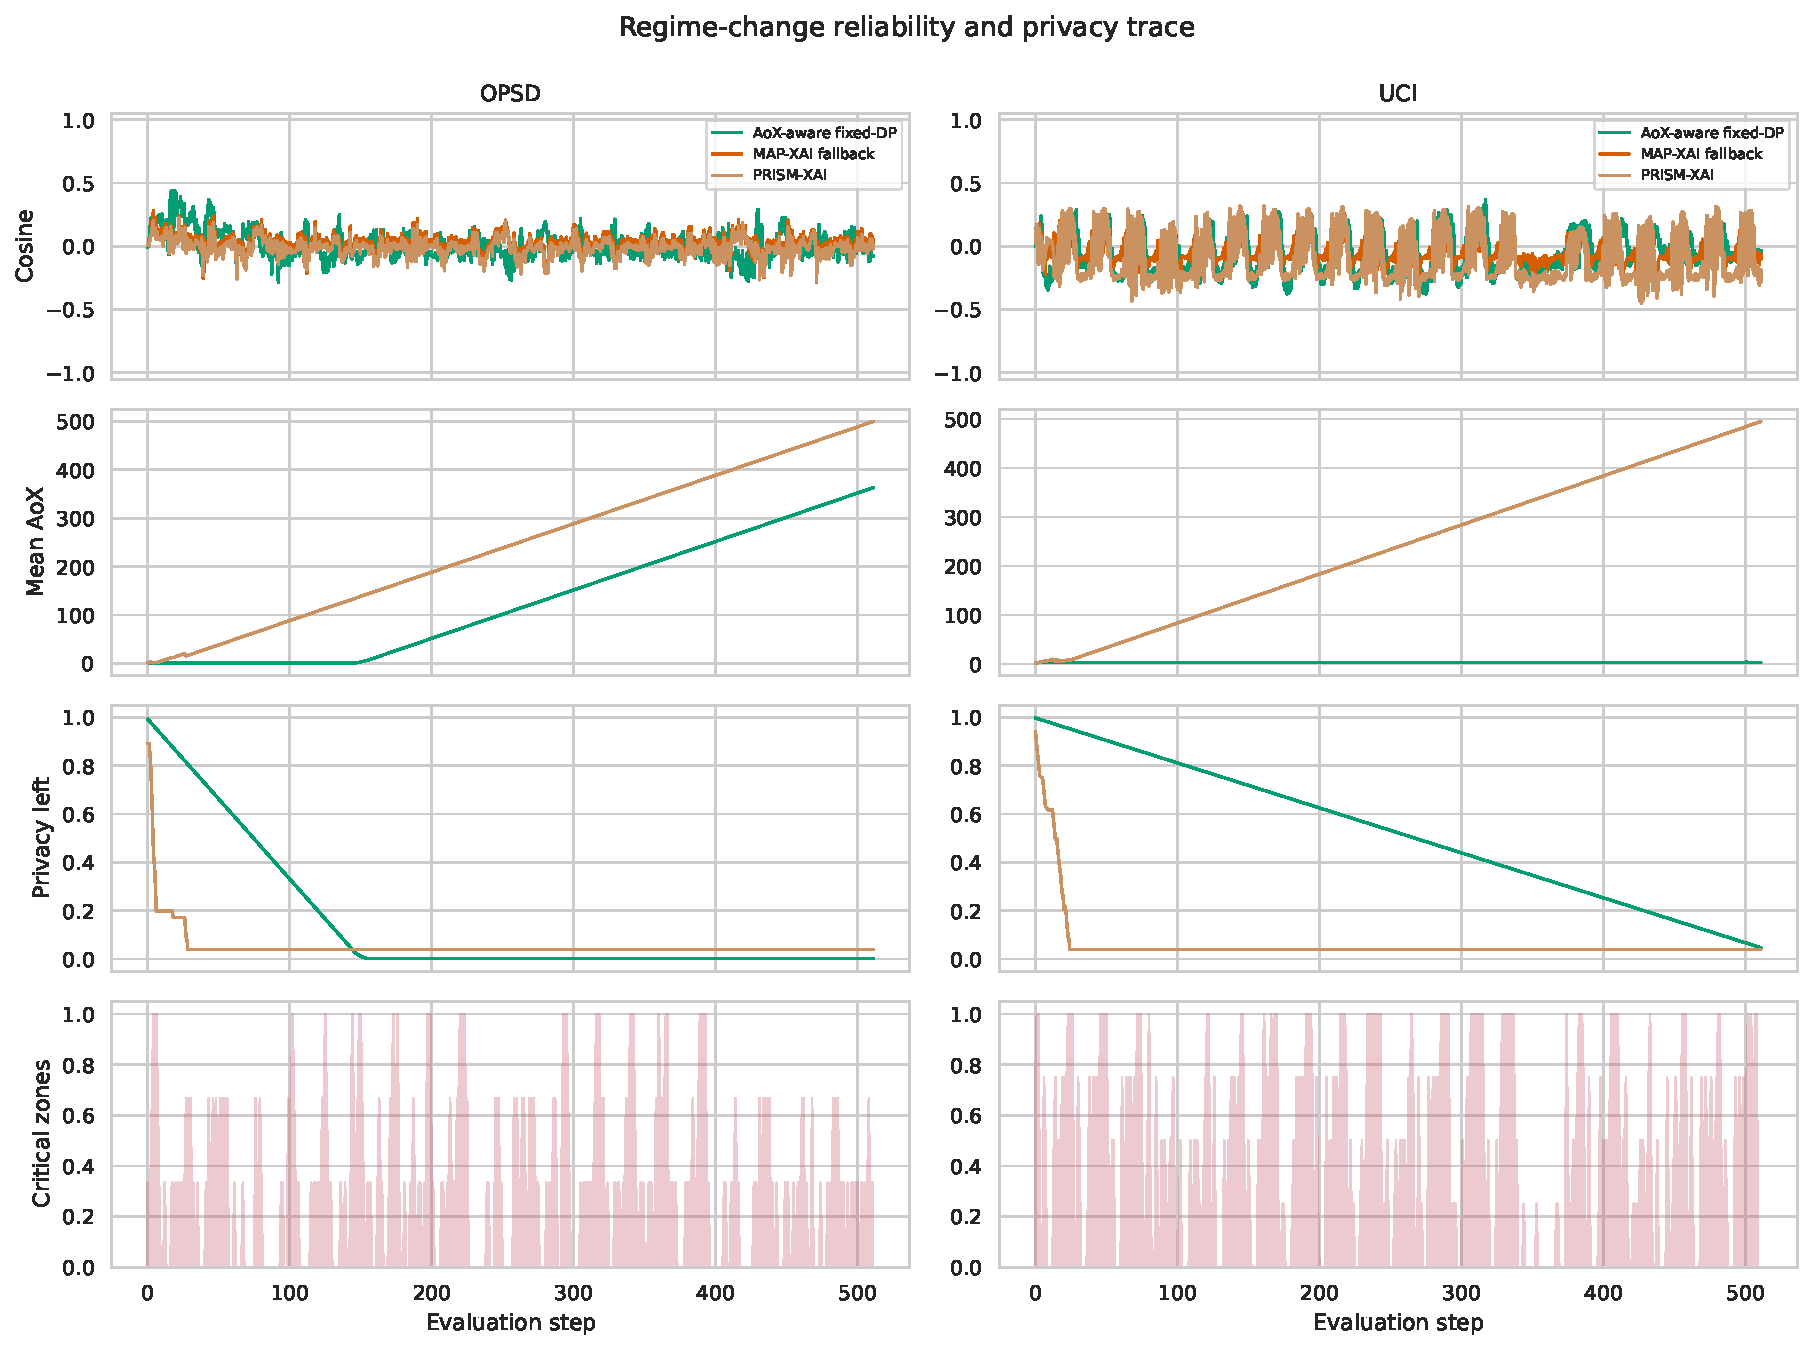
\includegraphics[width=0.96\textwidth,height=0.82\textheight,keepaspectratio]{supplementary_figures/residual_m4_combined_regime_trace.pdf}
\caption{Residual-score $M=4$, combined datasets: representative regime trace. The interpretation and claim boundary are given in the preceding subsection discussion.}
\end{figure*}
\clearpage

\begin{figure*}[p]
\centering
\includegraphics[width=0.96\textwidth,height=0.82\textheight,keepaspectratio]{supplementary_figures/residual_m4_combined_fairness_reliability.pdf}
\caption{Residual-score $M=4$, combined datasets: fairness and reliability. The interpretation and claim boundary are given in the preceding subsection discussion.}
\end{figure*}
\clearpage

\begin{figure*}[p]
\centering
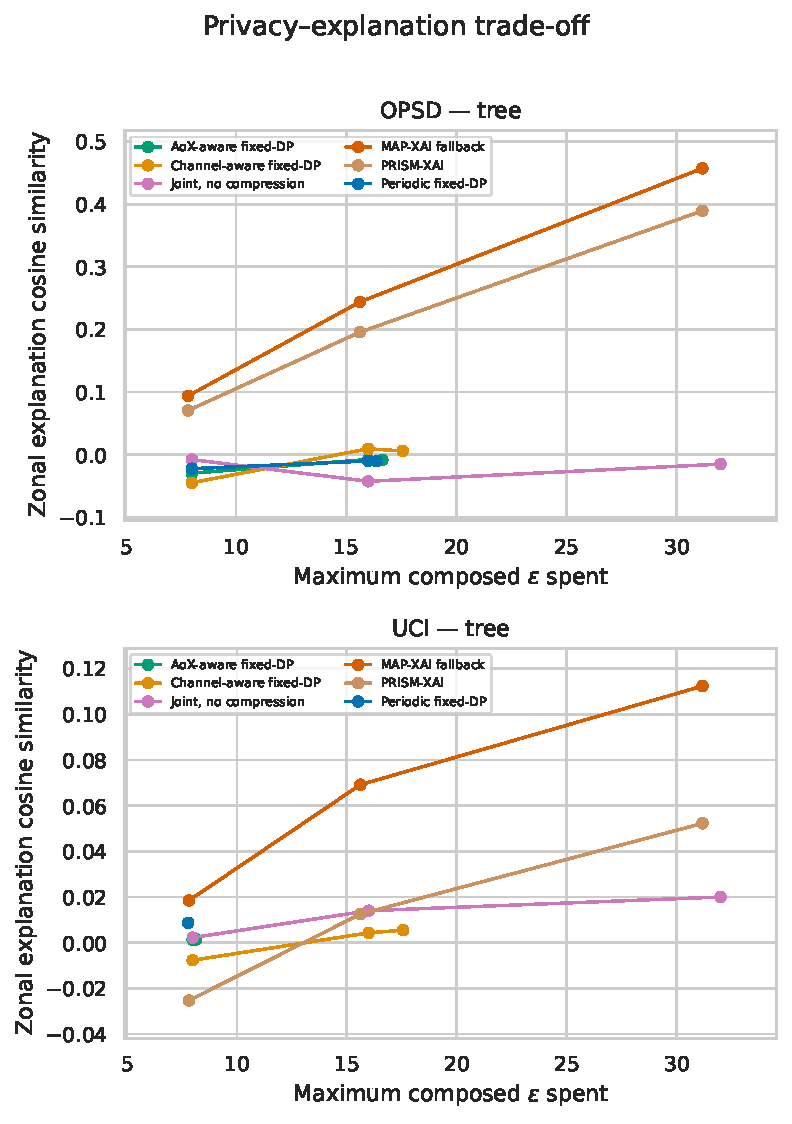
\includegraphics[width=0.96\textwidth,height=0.82\textheight,keepaspectratio]{supplementary_figures/residual_m4_combined_privacy_fidelity.pdf}
\caption{Residual-score $M=4$, combined datasets: privacy and fidelity. The interpretation and claim boundary are given in the preceding subsection discussion.}
\end{figure*}
\clearpage

\begin{figure*}[p]
\centering
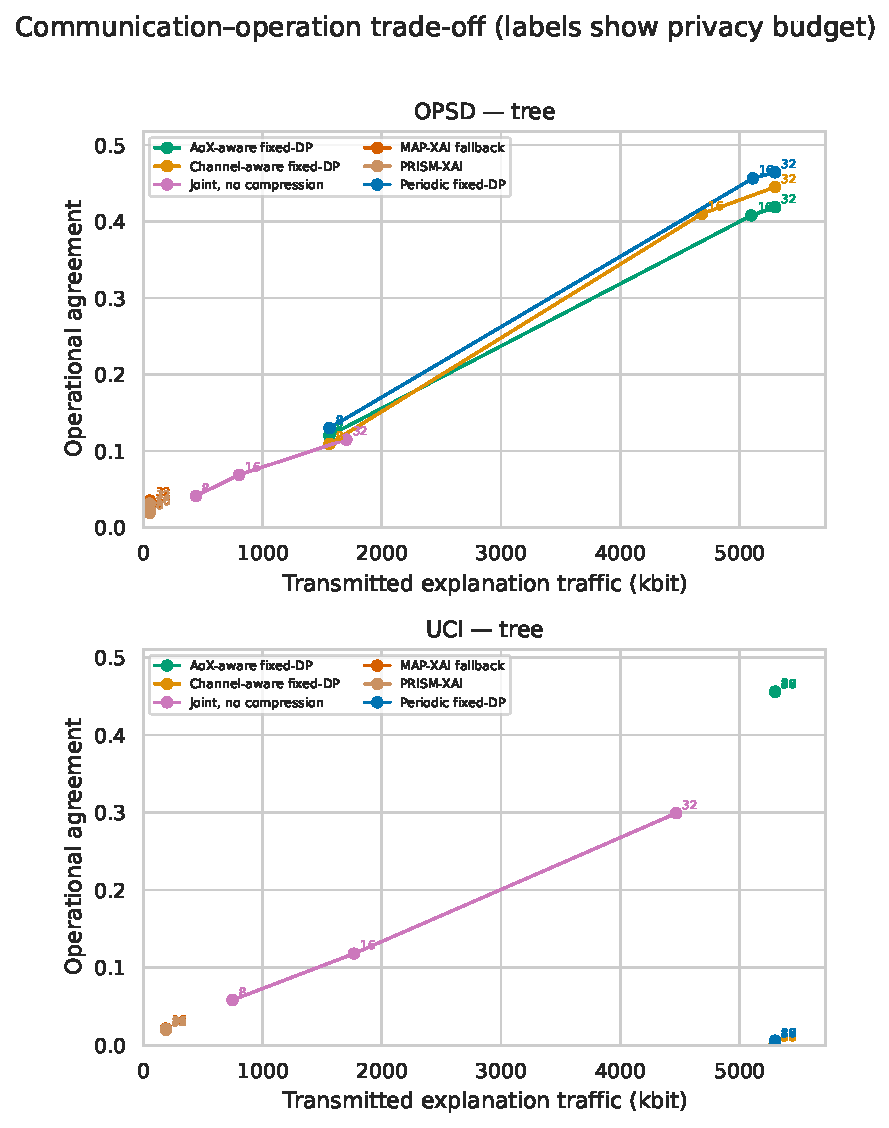
\includegraphics[width=0.96\textwidth,height=0.82\textheight,keepaspectratio]{supplementary_figures/residual_m4_combined_pareto_bits_fidelity.pdf}
\caption{Residual-score $M=4$, combined datasets: traffic--fidelity Pareto analysis. The interpretation and claim boundary are given in the preceding subsection discussion.}
\end{figure*}
\clearpage

\begin{figure*}[p]
\centering
\includegraphics[width=0.96\textwidth,height=0.82\textheight,keepaspectratio]{supplementary_figures/residual_m4_combined_ablation_results.pdf}
\caption{Residual-score $M=4$, combined datasets: ablation results. The interpretation and claim boundary are given in the preceding subsection discussion.}
\end{figure*}
\clearpage

\subsection{Residual-score $M=4$: OPSD}

For OPSD, the capped PRISM policy transmits approximately 52.1 kbit in the displayed conditions and abstains in about 95.5\% of opportunities. Coverage is about 0.045, lower than in the $M=8$ configuration, while the maximum composed expenditure remains close to the admitted horizon allowance. The low traffic therefore follows directly from stricter release scarcity and should not be presented independently of the reduced service rate.

The fidelity plots are comparatively favorable on OPSD: the paired Top-$K$ margin above random is $0.1000\pm0.0304$. The fairness panels show that the scarce releases are not concentrated on only a few endpoints, but high Jain fairness cannot compensate for limited coverage. The ablation panels show no robust incremental traffic benefit from adaptive resolution once the four-release cap is binding.

\begin{figure*}[p]
\centering
\includegraphics[width=0.96\textwidth,height=0.82\textheight,keepaspectratio]{supplementary_figures/residual_m4_opsd_regime_trace.pdf}
\caption{Residual-score $M=4$, OPSD: representative regime trace. The interpretation and claim boundary are given in the preceding subsection discussion.}
\end{figure*}
\clearpage

\begin{figure*}[p]
\centering
\includegraphics[width=0.96\textwidth,height=0.82\textheight,keepaspectratio]{supplementary_figures/residual_m4_opsd_fairness_reliability.pdf}
\caption{Residual-score $M=4$, OPSD: fairness and reliability. The interpretation and claim boundary are given in the preceding subsection discussion.}
\end{figure*}
\clearpage

\begin{figure*}[p]
\centering
\includegraphics[width=0.96\textwidth,height=0.82\textheight,keepaspectratio]{supplementary_figures/residual_m4_opsd_privacy_fidelity.pdf}
\caption{Residual-score $M=4$, OPSD: privacy and fidelity. The interpretation and claim boundary are given in the preceding subsection discussion.}
\end{figure*}
\clearpage

\begin{figure*}[p]
\centering
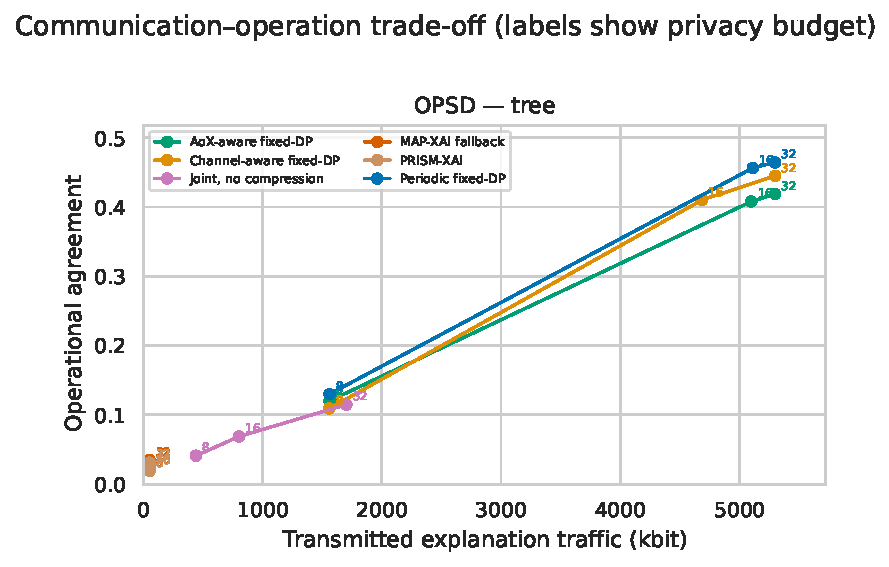
\includegraphics[width=0.96\textwidth,height=0.82\textheight,keepaspectratio]{supplementary_figures/residual_m4_opsd_pareto_bits_fidelity.pdf}
\caption{Residual-score $M=4$, OPSD: traffic--fidelity Pareto analysis. The interpretation and claim boundary are given in the preceding subsection discussion.}
\end{figure*}
\clearpage

\begin{figure*}[p]
\centering
\includegraphics[width=0.96\textwidth,height=0.82\textheight,keepaspectratio]{supplementary_figures/residual_m4_opsd_ablation_results.pdf}
\caption{Residual-score $M=4$, OPSD: ablation results. The interpretation and claim boundary are given in the preceding subsection discussion.}
\end{figure*}
\clearpage

\subsection{Residual-score $M=4$: UCI}

For UCI, capped PRISM traffic is about 189 kbit, again roughly half of the residual-$M=8$ level. Coverage falls to approximately 0.042--0.044 and abstention approaches 0.96. These plots characterize an intentionally sparse explanation channel rather than a high-availability monitoring service.

UCI Top-$K$ overlap is only $0.0197\pm0.0237$ above random and is not statistically detected after correction. The privacy--fidelity plane therefore shows no reliable fidelity benefit from the capped policy on this dataset. The fairness and trace panels are still useful systems diagnostics: they indicate even allocation and controlled expenditure, but do not establish that the received explanations are operationally useful.

\begin{figure*}[p]
\centering
\includegraphics[width=0.96\textwidth,height=0.82\textheight,keepaspectratio]{supplementary_figures/residual_m4_uci_regime_trace.pdf}
\caption{Residual-score $M=4$, UCI: representative regime trace. The interpretation and claim boundary are given in the preceding subsection discussion.}
\end{figure*}
\clearpage

\begin{figure*}[p]
\centering
\includegraphics[width=0.96\textwidth,height=0.82\textheight,keepaspectratio]{supplementary_figures/residual_m4_uci_fairness_reliability.pdf}
\caption{Residual-score $M=4$, UCI: fairness and reliability. The interpretation and claim boundary are given in the preceding subsection discussion.}
\end{figure*}
\clearpage

\begin{figure*}[p]
\centering
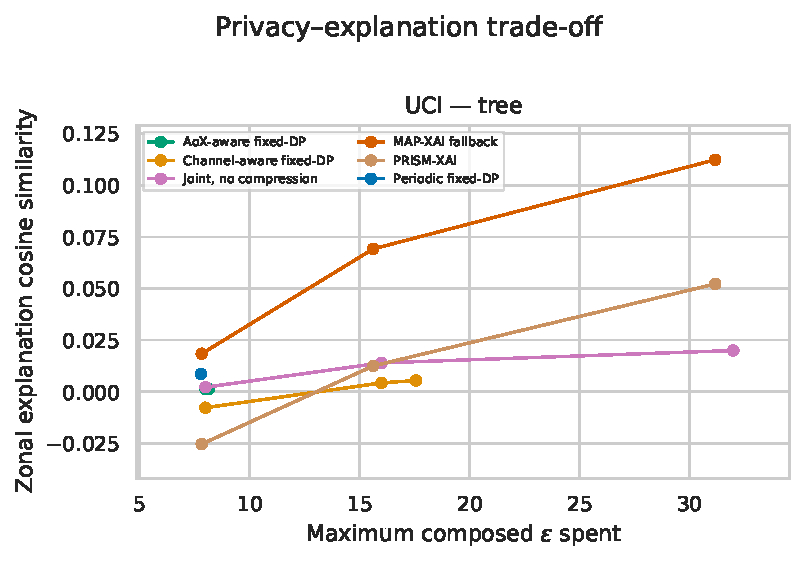
\includegraphics[width=0.96\textwidth,height=0.82\textheight,keepaspectratio]{supplementary_figures/residual_m4_uci_privacy_fidelity.pdf}
\caption{Residual-score $M=4$, UCI: privacy and fidelity. The interpretation and claim boundary are given in the preceding subsection discussion.}
\end{figure*}
\clearpage

\begin{figure*}[p]
\centering
\includegraphics[width=0.96\textwidth,height=0.82\textheight,keepaspectratio]{supplementary_figures/residual_m4_uci_pareto_bits_fidelity.pdf}
\caption{Residual-score $M=4$, UCI: traffic--fidelity Pareto analysis. The interpretation and claim boundary are given in the preceding subsection discussion.}
\end{figure*}
\clearpage

\begin{figure*}[p]
\centering
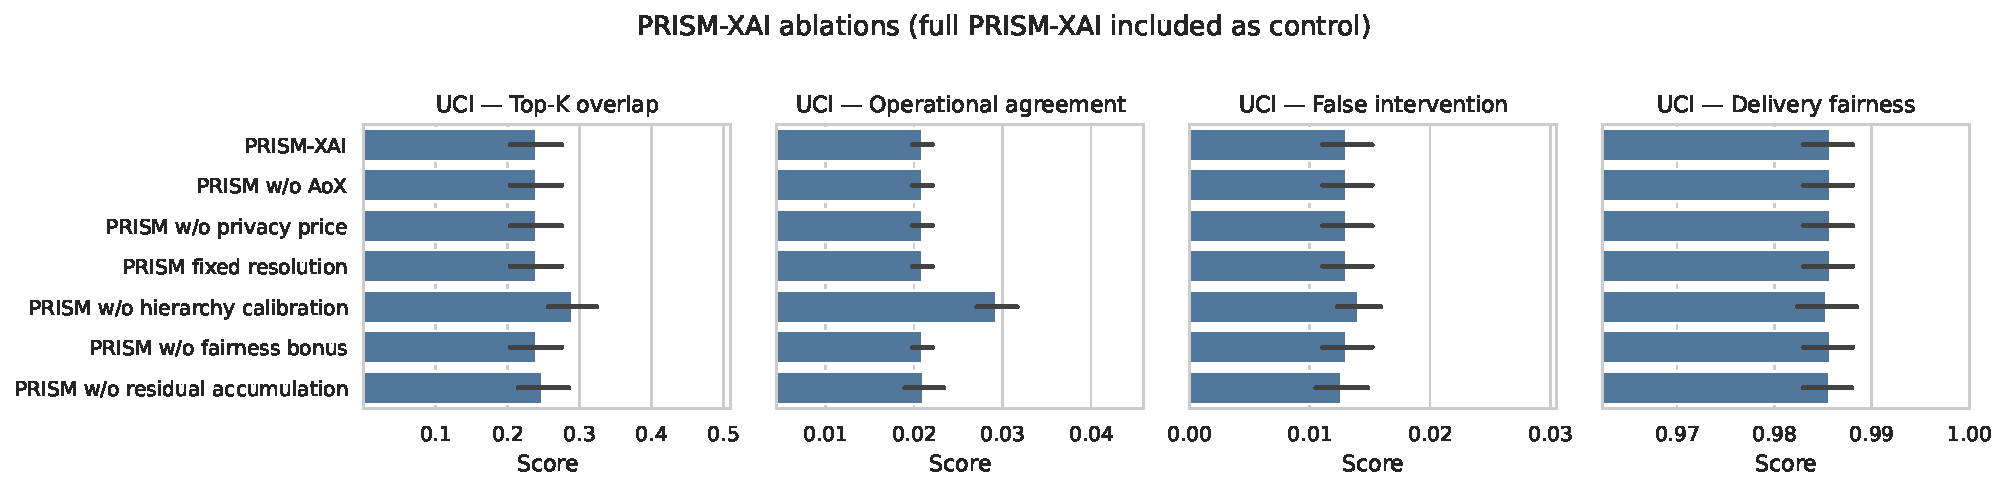
\includegraphics[width=0.96\textwidth,height=0.82\textheight,keepaspectratio]{supplementary_figures/residual_m4_uci_ablation_results.pdf}
\caption{Residual-score $M=4$, UCI: ablation results. The interpretation and claim boundary are given in the preceding subsection discussion.}
\end{figure*}
\clearpage

\subsection{Public-score $M=8$: combined datasets}

This is the primary configuration. Across 120 paired runs, PRISM-XAI transmits 207.31 kbit versus 243.71 kbit for MAP-XAI-only, a reduction of $36.40\pm3.32$ kbit or 15.72\%. Coverage changes by $-0.010$ percentage points, critical recall by $-0.083$ points, and recorded maximum privacy expenditure is unchanged. These are the conditions that support the paper's matched component claim.

The figure family shows why the public score matters. The regime traces schedule fewer packets without introducing a visible collapse in the paired service measures; the fairness panels keep the proposed method in the high-Jain region. The Pareto plot separates the matched MAP-XAI-only contrast from external fixed-DP policies that deliver different service. The adaptive-mode ablation accounts for a $35.33\pm5.63$ kbit saving (15.43\%), whereas fidelity, recall, and intervention-precision changes are not detected after BH correction. The combined Top-$K$ parametric result is positive, but its adjusted Wilcoxon result is not, so fidelity is interpreted by dataset below.

\begin{figure*}[p]
\centering
\includegraphics[width=0.96\textwidth,height=0.82\textheight,keepaspectratio]{supplementary_figures/public_m8_combined_regime_trace.pdf}
\caption{Public-score $M=8$, combined datasets: representative regime trace. The interpretation and claim boundary are given in the preceding subsection discussion.}
\end{figure*}
\clearpage

\begin{figure*}[p]
\centering
\includegraphics[width=0.96\textwidth,height=0.82\textheight,keepaspectratio]{supplementary_figures/public_m8_combined_fairness_reliability.pdf}
\caption{Public-score $M=8$, combined datasets: fairness and reliability. The interpretation and claim boundary are given in the preceding subsection discussion.}
\end{figure*}
\clearpage

\begin{figure*}[p]
\centering
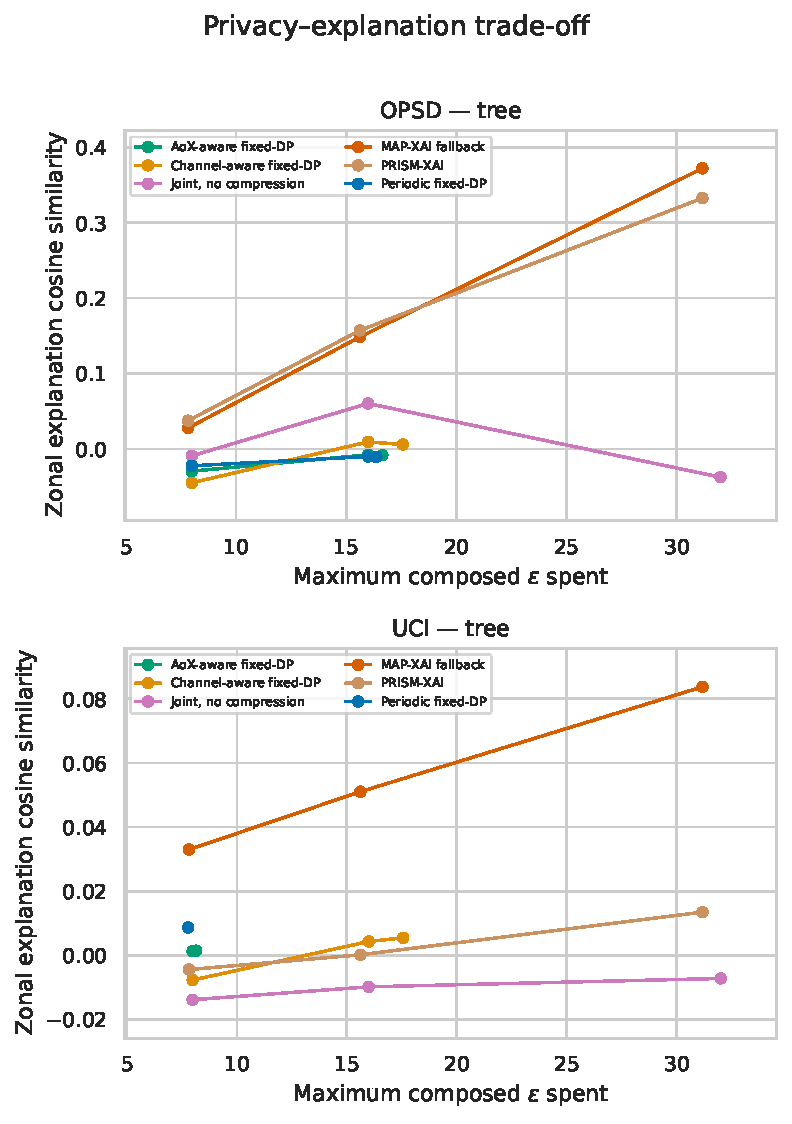
\includegraphics[width=0.96\textwidth,height=0.82\textheight,keepaspectratio]{supplementary_figures/public_m8_combined_privacy_fidelity.pdf}
\caption{Public-score $M=8$, combined datasets: privacy and fidelity. The interpretation and claim boundary are given in the preceding subsection discussion.}
\end{figure*}
\clearpage

\begin{figure*}[p]
\centering
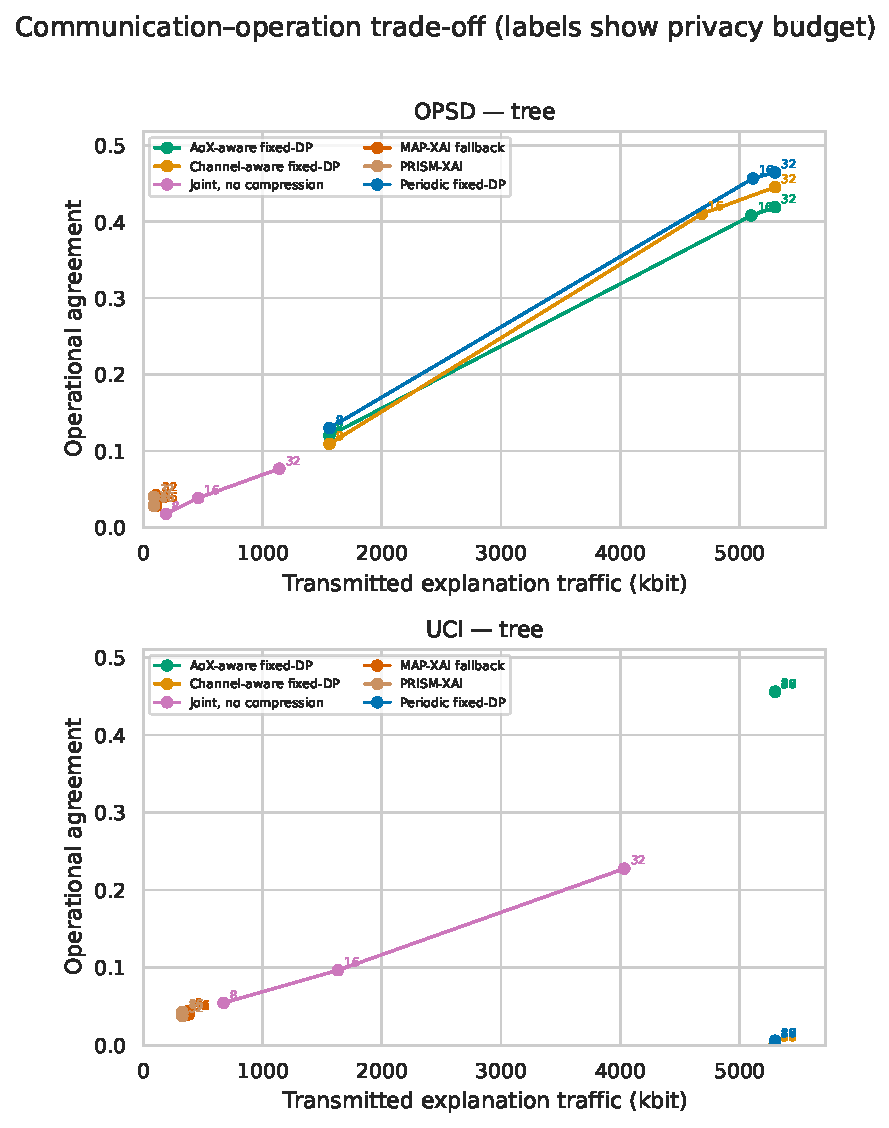
\includegraphics[width=0.96\textwidth,height=0.82\textheight,keepaspectratio]{supplementary_figures/public_m8_combined_pareto_bits_fidelity.pdf}
\caption{Public-score $M=8$, combined datasets: traffic--fidelity Pareto analysis. The interpretation and claim boundary are given in the preceding subsection discussion.}
\end{figure*}
\clearpage

\begin{figure*}[p]
\centering
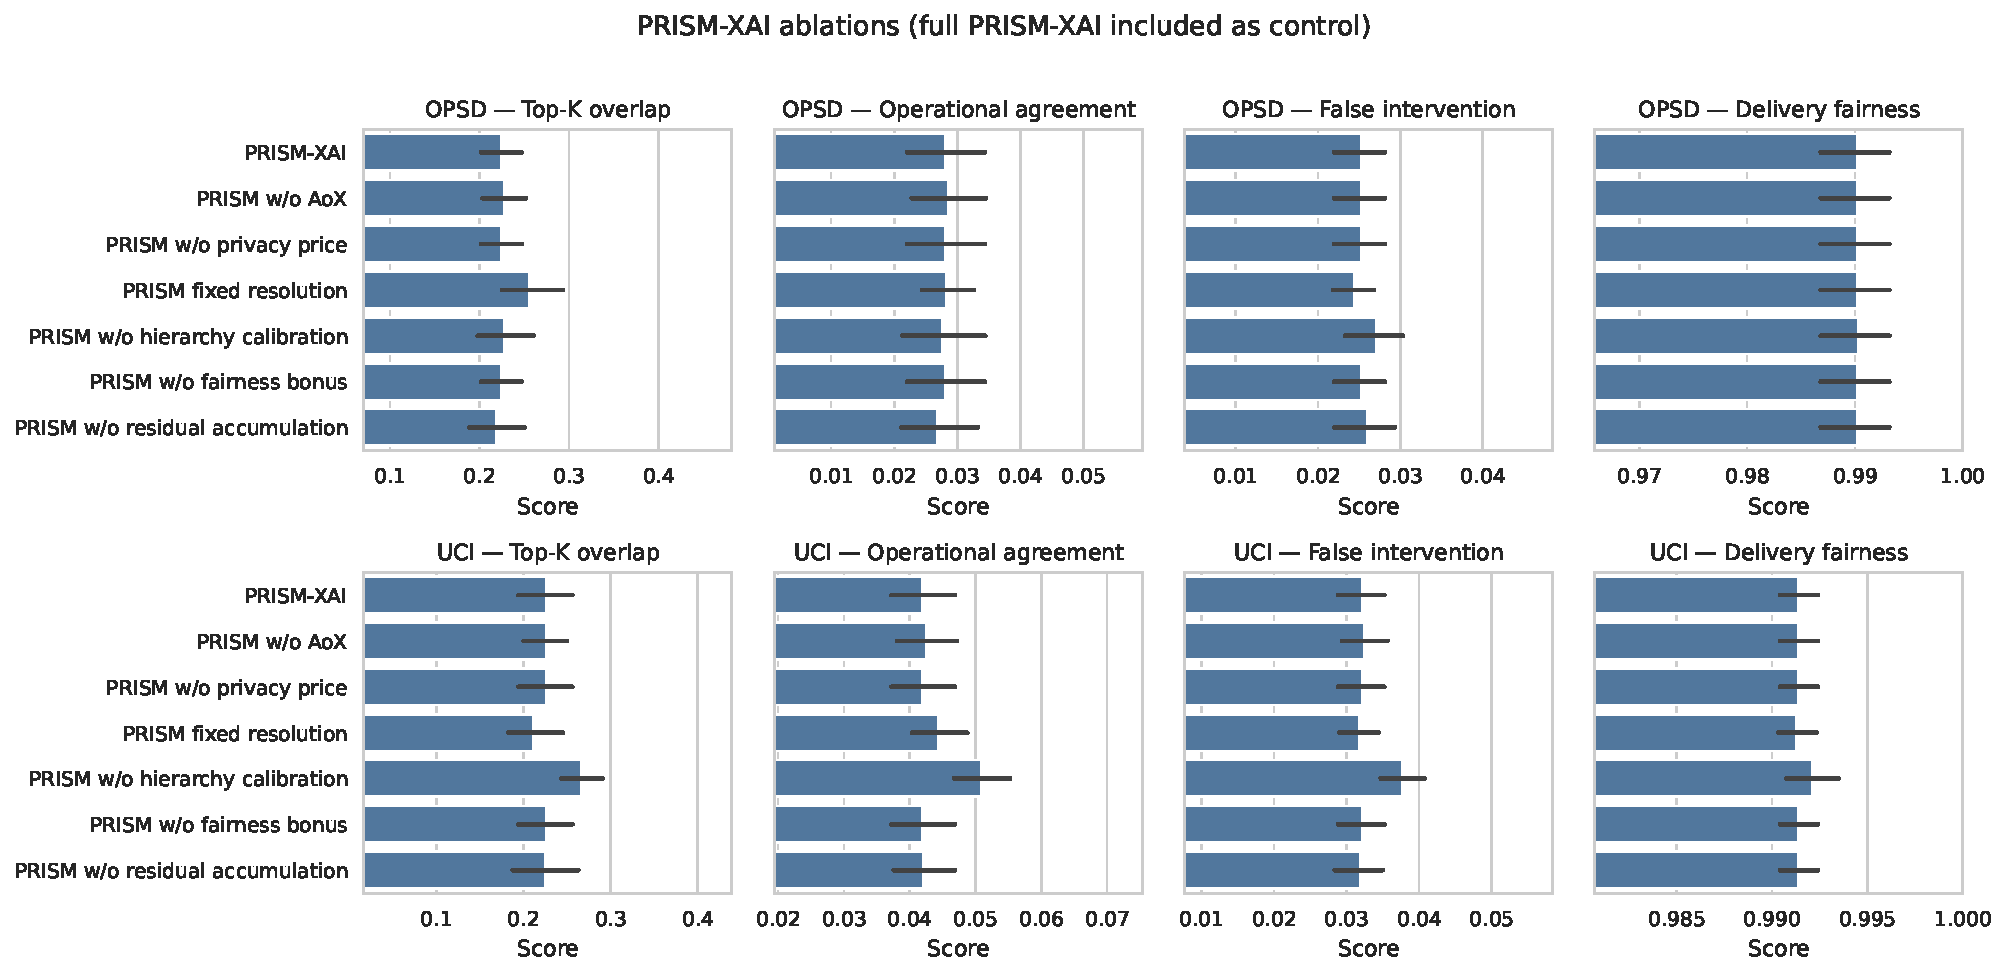
\includegraphics[width=0.96\textwidth,height=0.82\textheight,keepaspectratio]{supplementary_figures/public_m8_combined_ablation_results.pdf}
\caption{Public-score $M=8$, combined datasets: ablation results. The interpretation and claim boundary are given in the preceding subsection discussion.}
\end{figure*}
\clearpage

\subsection{Public-score $M=8$: OPSD}

On OPSD, the primary PRISM configuration averages 87.98 kbit compared with 106.15 kbit for MAP-XAI-only in the dataset-level summary. Coverage remains about 0.071 and critical recall changes only slightly. This establishes that a meaningful portion of the aggregate traffic reduction occurs even in the smaller nine-endpoint setting.

OPSD also supplies the positive fidelity evidence: Top-$K$ overlap exceeds random by $0.0435\pm0.0243$, with adjusted Wilcoxon $q=0.0089$. The privacy--fidelity panel nevertheless shows that agreement varies across explainers and budgets, so the result is a measured proxy rather than a universal semantic guarantee. The traces demonstrate sparse public-state scheduling, and the ablations show that the gain is associated with adaptive public-score mode selection rather than a lower release cap.

\begin{figure*}[p]
\centering
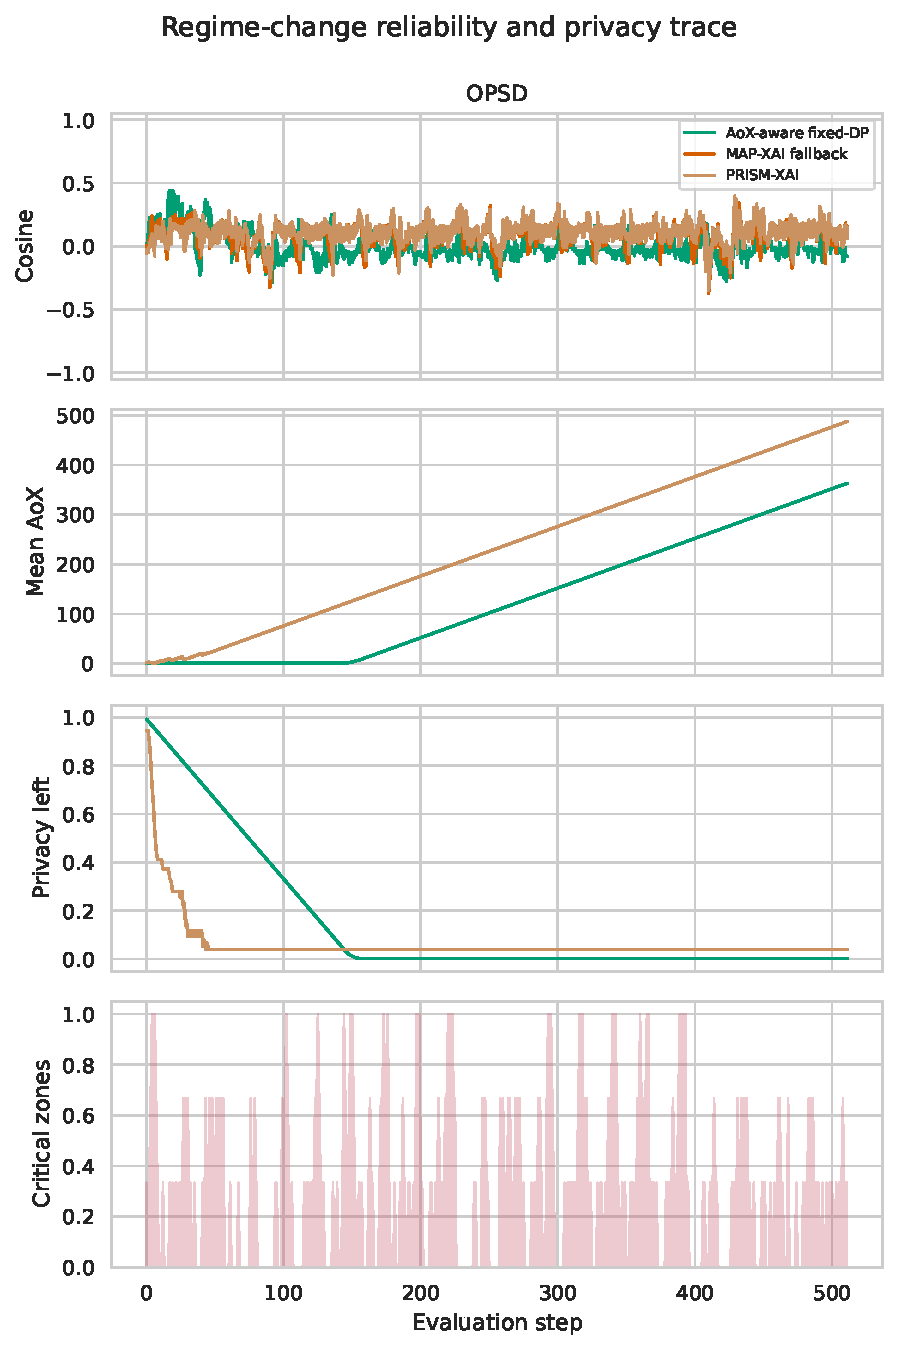
\includegraphics[width=0.96\textwidth,height=0.82\textheight,keepaspectratio]{supplementary_figures/public_m8_opsd_regime_trace.pdf}
\caption{Public-score $M=8$, OPSD: representative regime trace. The interpretation and claim boundary are given in the preceding subsection discussion.}
\end{figure*}
\clearpage

\begin{figure*}[p]
\centering
\includegraphics[width=0.96\textwidth,height=0.82\textheight,keepaspectratio]{supplementary_figures/public_m8_opsd_fairness_reliability.pdf}
\caption{Public-score $M=8$, OPSD: fairness and reliability. The interpretation and claim boundary are given in the preceding subsection discussion.}
\end{figure*}
\clearpage

\begin{figure*}[p]
\centering
\includegraphics[width=0.96\textwidth,height=0.82\textheight,keepaspectratio]{supplementary_figures/public_m8_opsd_privacy_fidelity.pdf}
\caption{Public-score $M=8$, OPSD: privacy and fidelity. The interpretation and claim boundary are given in the preceding subsection discussion.}
\end{figure*}
\clearpage

\begin{figure*}[p]
\centering
\includegraphics[width=0.96\textwidth,height=0.82\textheight,keepaspectratio]{supplementary_figures/public_m8_opsd_pareto_bits_fidelity.pdf}
\caption{Public-score $M=8$, OPSD: traffic--fidelity Pareto analysis. The interpretation and claim boundary are given in the preceding subsection discussion.}
\end{figure*}
\clearpage

\begin{figure*}[p]
\centering
\includegraphics[width=0.96\textwidth,height=0.82\textheight,keepaspectratio]{supplementary_figures/public_m8_opsd_ablation_results.pdf}
\caption{Public-score $M=8$, OPSD: ablation results. The interpretation and claim boundary are given in the preceding subsection discussion.}
\end{figure*}
\clearpage

\subsection{Public-score $M=8$: UCI}

On UCI, PRISM-XAI averages 326.63 kbit compared with 381.26 kbit for MAP-XAI-only. Because UCI contains 32 endpoints, its absolute traffic is higher than OPSD, and it contributes the larger absolute share of the combined reduction. Coverage remains near 0.085--0.090 and critical recall near 0.041, so the comparison remains within the declared matched region.

The UCI fidelity result remains the principal caution. Top-$K$ overlap differs from random by $-0.0050\pm0.0216$, with no adjusted statistical support. The traffic and fairness figures therefore establish resource-allocation behavior, not explanation usefulness. The Pareto and ablation panels show that public-score scheduling can remove traffic while preserving the tested service proxies, but a task-grounded or operator study is still required before treating these packets as actionable explanations.

\begin{figure*}[p]
\centering
\includegraphics[width=0.96\textwidth,height=0.82\textheight,keepaspectratio]{supplementary_figures/public_m8_uci_regime_trace.pdf}
\caption{Public-score $M=8$, UCI: representative regime trace. The interpretation and claim boundary are given in the preceding subsection discussion.}
\end{figure*}
\clearpage

\begin{figure*}[p]
\centering
\includegraphics[width=0.96\textwidth,height=0.82\textheight,keepaspectratio]{supplementary_figures/public_m8_uci_fairness_reliability.pdf}
\caption{Public-score $M=8$, UCI: fairness and reliability. The interpretation and claim boundary are given in the preceding subsection discussion.}
\end{figure*}
\clearpage

\begin{figure*}[p]
\centering
\includegraphics[width=0.96\textwidth,height=0.82\textheight,keepaspectratio]{supplementary_figures/public_m8_uci_privacy_fidelity.pdf}
\caption{Public-score $M=8$, UCI: privacy and fidelity. The interpretation and claim boundary are given in the preceding subsection discussion.}
\end{figure*}
\clearpage

\begin{figure*}[p]
\centering
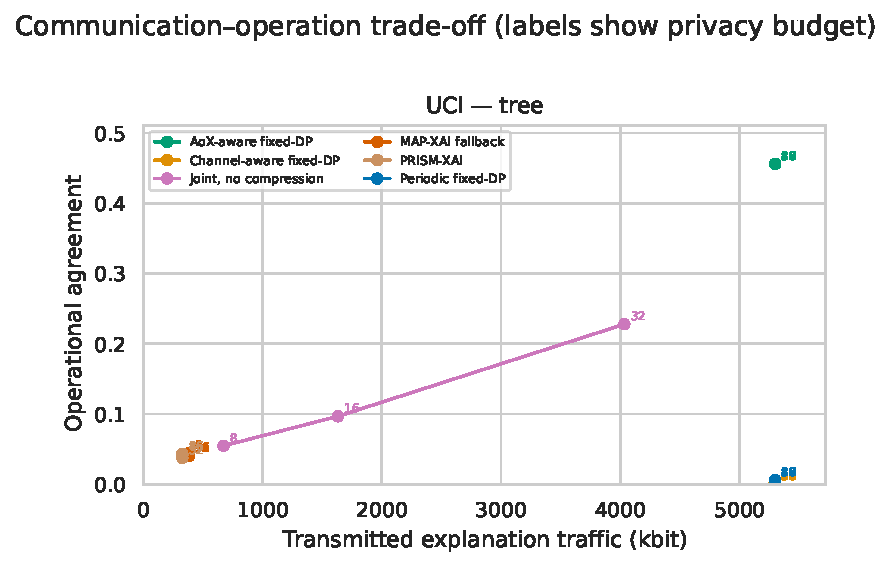
\includegraphics[width=0.96\textwidth,height=0.82\textheight,keepaspectratio]{supplementary_figures/public_m8_uci_pareto_bits_fidelity.pdf}
\caption{Public-score $M=8$, UCI: traffic--fidelity Pareto analysis. The interpretation and claim boundary are given in the preceding subsection discussion.}
\end{figure*}
\clearpage

\begin{figure*}[p]
\centering
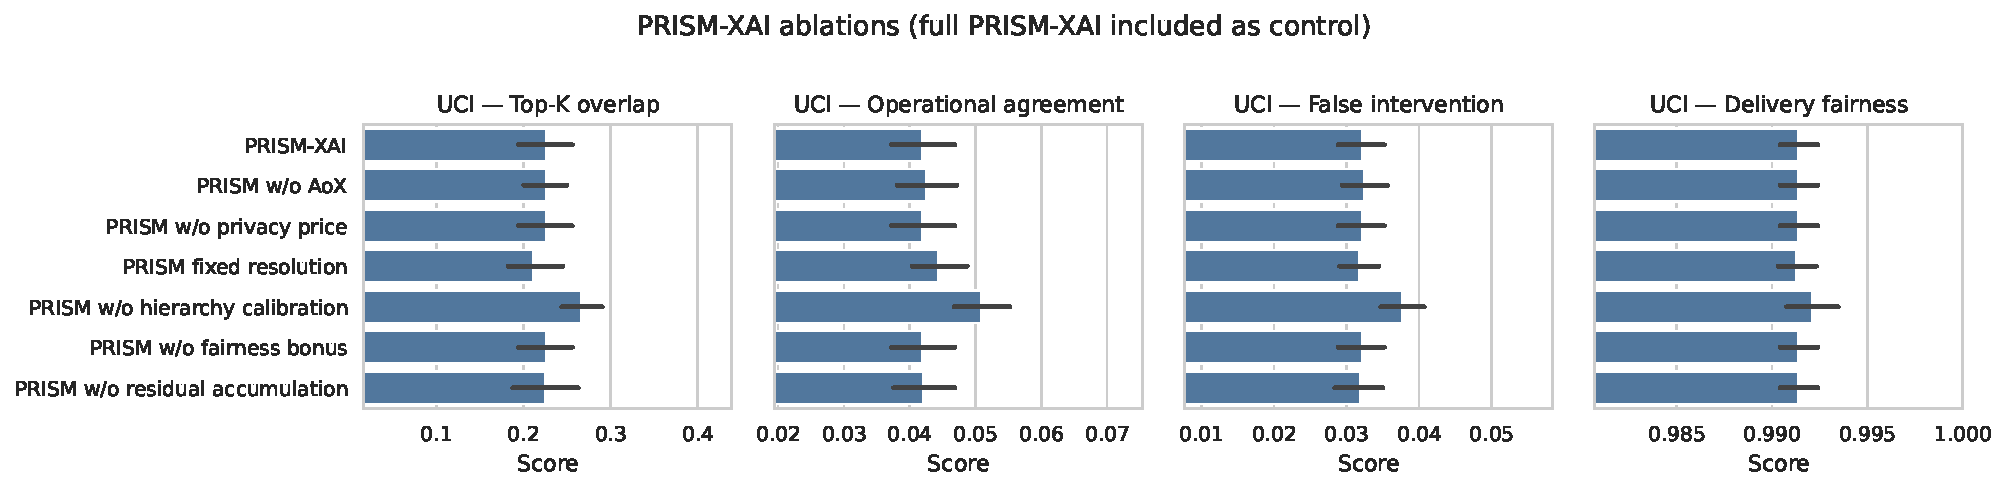
\includegraphics[width=0.96\textwidth,height=0.82\textheight,keepaspectratio]{supplementary_figures/public_m8_uci_ablation_results.pdf}
\caption{Public-score $M=8$, UCI: ablation results. The interpretation and claim boundary are given in the preceding subsection discussion.}
\end{figure*}
\clearpage
